\documentclass{article}


% if you need to pass options to natbib, use, e.g.:
%     \PassOptionsToPackage{numbers, compress}{natbib}
% before loading neurips_2024


% ready for submission
\usepackage{neurips_2024}


% to compile a preprint version, e.g., for submission to arXiv, add add the
% [preprint] option:
%     \usepackage[preprint]{neurips_2024}


% to compile a camera-ready version, add the [final] option, e.g.:
%     \usepackage[final]{neurips_2024}


% to avoid loading the natbib package, add option nonatbib:
%    \usepackage[nonatbib]{neurips_2024}


\usepackage[utf8]{inputenc} % allow utf-8 input
\usepackage[T1]{fontenc}    % use 8-bit T1 fonts
\usepackage{hyperref}       % hyperlinks
\usepackage{url}            % simple URL typesetting
\usepackage{booktabs}       % professional-quality tables
\usepackage{amsfonts}       % blackboard math symbols
\usepackage{nicefrac}       % compact symbols for 1/2, etc.
\usepackage{microtype}      % microtypography
\usepackage{xcolor}         % colors

\usepackage{orcidlink}
\usepackage{graphicx}
\usepackage{amsmath}
\usepackage{amssymb}
\usepackage{booktabs}
\usepackage{algorithm}
\usepackage{algpseudocode}
\usepackage{graphicx}
\usepackage{booktabs}

% Define the title
\title{Communication-Efficient \& Class-Balancing Federated Learning with Adaptive Consensus Dropout \& Model Quantization}

% Define the author(s)
\author{%
  Shaif Chowdhury \\
  Computer Science Department\\
  Baylor University\\
  \texttt{Shaif_chowdhury1@baylor.edu} \\
  \And
  Aaron Carney \\
  Computer Science Department\\
  Baylor University\\
  \texttt{Aaron_carney1@baylor.edu} \\
}

\begin{document}
\maketitle


% The \author macro works with any number of authors. There are two commands
% used to separate the names and addresses of multiple authors: \And and \AND.
%
% Using \And between authors leaves it to LaTeX to determine where to break the
% lines. Using \AND forces a line break at that point. So, if LaTeX puts 3 of 4
% authors names on the first line, and the last on the second line, try using
% \AND instead of \And before the third author name.


\begin{abstract}

Federated learning(FL) is used to train deep learning models over over heterogeneous and decentralized datasets. Communication between client and server can be a major bottleneck for FL, specially in case of large models. More over there is often data imbalance issue in real world FL problems. 

To address these issues, we propose a novel, balanced, communication-efficient FL strategy. Our strategy is based on two key elements: a novel adaptive voting-based federated dropout on client models addressing both communication bottlenecks and data imbalance, and a quantization method to improve communication efficiency. We empirically demonstrate that the combination of these two strategies enhances the communication strategy while improving the accuracy of the model across several datasets and experimental settings. We get around 7x reduction in communication cost without degrading the quality of the model. Our code can be found at \url{https://anonymous.4open.science/r/Federated_lr-2140/}.


\end{abstract}

\section{Introduction}

\subsection{Motivation for Federated Learning}

The digital era is witnessing an unprecedented increase in data generation, much of which is highly sensitive and personal. This surge necessitates the advancement of deep learning models that can be trained over decentralized and heterogeneous datasets, thus ushering in the era of FL. FL represents a paradigm shift from traditional centralized machine learning approaches by enabling the training of models directly on devices where the data is generated \cite{info13050263}. This method ensures data privacy since the raw data never leaves its original device, thereby addressing growing concerns over data security and privacy in the age of information\cite{mao2022communication, zhang2022homomorphic}.\par

The cornerstone of FL lies in its ability to maintain the confidentiality and integrity of data. In traditional machine learning approaches, data aggregation poses significant risks of privacy breaches. However, FL aims to circumvent this issue by decentralizing the data processing, thereby safeguarding sensitive information. This approach can not only enhances user trust but also complies with stringent data protection regulations such as the General Data Protection Regulation (GDPR) in Europe \cite{team2020eu}.\par

While FL presents an innovative solution to privacy concerns, it introduces unique challenges stemming from the decentralized nature of data. These challenges include managing data heterogeneity across different devices and ensuring model performance despite the varying quality and quantity of local datasets. The decentralized framework of FL necessitates novel approaches to model training and aggregation to tackle these obstacles efficiently while maintaining the aforementioned privacy tenets \cite{li2021fedsae}.\par

\subsection{Challenges in Federated Learning}

\subsubsection{Communication Bottleneck}
One of the paramount challenges in FL is the communication bottleneck that arises, especially with large deep learning models. The necessity to frequently exchange model updates between the server and numerous clients can lead to significant communication overhead \cite{nader2020adaptive}. This issue is exacerbated in scenarios with limited bandwidth or when the model size becomes substantially large, thereby straining network resources and impacting the efficiency of the learning process.\par

\subsubsection{Data Imbalance}
Another significant challenge is the inherent data imbalance across clients in FL settings. Given that data is generated in a non-IID (independent and identically distributed) manner across different devices, some clients may have more data or more diverse data than others. This imbalance can lead to skewed model updates, where the model disproportionately learns from clients with more or more varied data, potentially compromising the overall model performance and fairness \cite{10.1093/comjnl/bxac118, jeon2024federated}.\par

\subsubsection{Proposed Solution}

Neural Network quantization techniques can play a critical role in mitigating communication bottlenecks. While regularization methods like dropout can improve model performance as well as improve communication efficiency \cite{srivastava2014dropout}. Dropout works by  randomly "dropping out" (setting to zero) a certain percentage of neural network units during the training. When combined with an appropriate quantization method dropout can significantly reduce the amount of data transmission between client and server. Such reduction is vital for the efficient transmission of model updates over networks with limited bandwidth \cite{10472332}. Furthermore, incorporating dropout can also serve as an effective regularization technique. It improves model robustness against over-fitting and enhances its generalization capabilities across decentralized datasets \cite{srivastava2014dropout,pezoulas2024fhbf}.\par

Furthermore, the application of dropout and quantization techniques can inadvertently bolster the security of FL systems. By reducing the model's complexity, the potential attack surface for adversarial attacks is minimized, thereby safeguarding both the integrity of the model and the privacy of user data \cite{TANG2024269}. This dual benefit underscores the importance of model compression not only for improving FL efficiency and scalability but also for reinforcing the security posture of FL ecosystems against evolving cyber-security threats.\par

\begin{figure*}[h]
  \centering
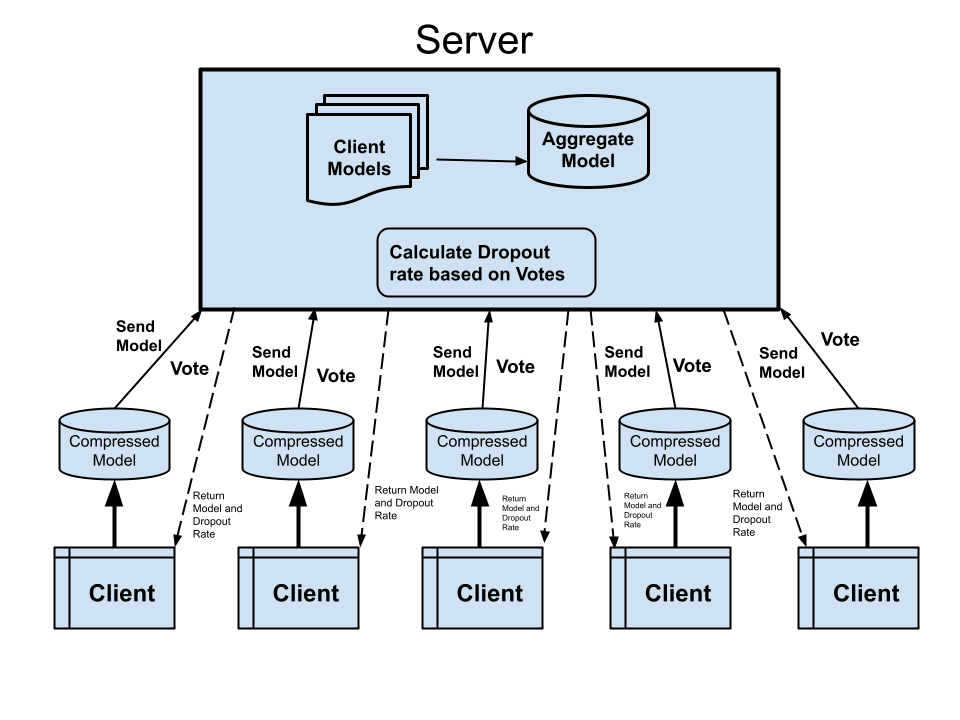
\includegraphics[width = 0.7\textwidth, height = .55\linewidth]{img/1.Fed_Lr.png}
\caption{A block diagram of ACFed learning with Quantization.}
  \label{fig:fed_lr}
\end{figure*}

In this paper, we propose two novel strategies to mitigate the communication footprint in FL and provide empirical evidence demonstrating that our model is robust to data imbalance. The specific contributions of this study are as follows:

\textbf{Adaptive Consensus Federated Dropout (ACFed)} innovates by integrating the conventional Dropout \cite{srivastava2014dropout} technique, previously proposed federated dropout \cite{wen2022federated} with and a voting based adaptive dropout method inspired by CLIMB Algorithm \cite{shen2021agnostic}. Our method involves training client models that start with a fixed dropout rate, but adjust this rate dynamically based on model performance feedback from the server. The clients vote to either increase or decrease the dropout and based on that server makes a decision. If a client model achieves higher accuracy than what the server model returns, then it votes to increase the dropout rate; conversely, it votes to decrease if the server's model performs better.\par

\textbf{Model Quantization} forms our second approach to reducing the communication footprint in FL environments significantly. By implementing various quantization levels introduced before \cite{jacob2018quantization}, from float16 to int8, this method efficiently lowers bandwidth requirements while negligibly affecting model performance. Our experiments across multiple benchmark datasets showcase the robustness of model quantization, particularly when combined with adaptive dropout techniques, even on datasets with class imbalances like imbalanced-cifar.\par

\textbf{Empirical Validation} through experiments on several benchmark datasets confirms the effectiveness of our proposed strategies. The combined use of ACFed and model quantization not only conserves bandwidth but also proves robust against class imbalances, thereby providing a compelling case for their application in practical FL scenarios. We also provide our source-code with examples to make it easy to integrate our method with existing FL frameworks and different model architectures.\par

\section{Related Work}

\subsection{Foundations of Federated Learning} 
FL has emerged as a paradigm that leverages vast, dispersed datasets while ensuring privacy protection. Originating from the work of McMahan et al.\cite{DBLP:journals/corr/McMahanMRA16} in 2016, FL enables model training across multiple devices without centralizing data, thus addressing the privacy and security limitations of traditional cloud-based methods. By decentralizing the process, FL enhances privacy and reduces the bandwidth needed for data transfer, a significant advantage in the era of rapid digital expansion \cite{ijerph20156539}.

At the core of FL are principles of collaborative model training. Data remains on local devices and only model updates are shared with a central server. This server aggregates updates to improve the global model and then distributes the result back to the devices for further training \cite{Li_2020}. Through iterative cycles, the model enhances using diverse data sources while maintaining data privacy, aligning with strict regulations such as GDPR \cite{team2020eu}.

A key development in FL was the creation of the FederatedAveraging algorithm (FedAvg) by McMahan et al \cite{DBLP:journals/corr/abs-1710-06963}, which reduces communication overhead and speeds up model convergence by averaging local updates, optimizing both efficiency and effectiveness. Subsequent FL research has tackled challenges like non-IID data, system heterogeneity, and defense against adversarial attacks. Notable contributions include Konečný et al\cite{konevcny2016federated} methods for efficient communication.

\subsection{Communication Efficiency and Quantization}

FL signifies a substantial shift in machine learning by decentralizing data processing, thus enhancing data privacy and security. This transformation introduces a critical challenge: ensuring communication efficiency. Aggregating updates from numerous devices to a central server can be bandwidth-intensive and slow, particularly as machine learning models grow in complexity \cite{li2023pbfl}.

To achieve communication efficiency, FL strategies focus on reducing bandwidth and latency during large-scale model update transmissions \cite{li2023pbfl}. Essential methods include pruning, and compression techniques, all aimed at decreasing the data volume communicated. Quantization, a form of compression, reduces the precision of model parameters, significantly lessens data transmission volume while only marginally affecting model accuracy depending on implementation\cite{jacob2018quantization}.

Quantization in FL has evolved from basic probabilistic approaches for model weight reduction \cite{konevcny2016federated} to more sophisticated methods. Initial research such as that by Benoit et al. \cite{jacob2018quantization} in 2018 highlighted the limitations of early over-parameterized proofs of concept. Recent methodologies, like QuPeD \cite{ozkara2021quped}, innovate by integrating distillation with vector quantization, enhancing precision over scalar alternatives. Further exploration into vector quantization has been pursued through various frameworks including UVeQFed \cite{shlezinger2020uveqfed}, HeteroSAg \cite{elkordy2022heterosag}, JoPEQ \cite{lang2023joint}, and the latest, FedVQCS \cite{oh2023fedvqcs}. Additionally, approaches such as T-FedAvg \cite{xu2020ternary} utilize ternary quantization to simplify weights to -1, 0, 1. Innovations continue with non-uniform \cite{chen2024communication} and stochastic quantization, which employs random rounding to mitigate the constraints of traditional deterministic methods \cite{li2022federated}.

\subsection{Addressing Data Imbalance}
Data imbalance refers to scenarios where data across various nodes are unevenly distributed, either in quantity or in quality. This uneven distribution can significantly skew the learning model, as nodes with fewer data samples—often containing minority representations—might be underrepresented in the training of the global model. Consequently, this leads to biased or inadequate generalizations when the model is subsequently applied to unseen data. Such imbalances pose a critical challenge in developing robust machine learning models that perform well across diverse datasets.

Data Distribution Management encompasses strategies that adjust the distribution of data across nodes to enhance model equity. Techniques include Re-balancing Techniques and Transfer Learning \cite{Sakho2024TheoreticalAE, lin2017clustering}. Algorithmic modifications aim to refine learning processes to handle imbalanced data better by modifying optimization objectives to emphasize minority classes, integrating fairness to reduce biases across nodes \cite{inproceedings}, and implementing regularization methods such as dropout to mitigate over-fitting and manage disparities in data \cite{pezoulas2024fhbf}. Additional methodologies, such as anomaly detection, re-calibrate focus towards underrepresented data \cite{Singh2020AnomalyDU}, while inherently adaptive strategies like meta-learning\cite{hospedales2021meta,huisman2021survey} and multi-task learning\cite{mills2021multi} are tailored to optimize performance based on the unique distributions at each node.\par

\subsection{Dropout Techniques}
Dropout in the traditional definition has likewise developed many avenues of research. Some models fall under the type of global dropout, which is where all clients have the same technique applied to them. The other side is called local dropout, or sometimes sub-model learning \cite{jia2022x}. Local dropout is where partitions of the network are given differential parameters for dropout. This differentiation is an operational one and often times whether in the same study or different ones, the same techniques are often applied in both the global and local form.

Some techniques include using randomness as part or most of the process\cite{wen2022federated}, FedDrop is notable example. Other techniques use Bayesian Inference-based Dropout \cite{gal2016theoretically, xue2023fedbiad}, FjORD \cite{horvath2021fjord} is a seminal example, dropping partial back rows in weight matrices, which places pike-and-slab distributions over weights. Other techniques use design score maps like AFD \cite{nader2020adaptive}, an early adaptive technique. Still others use differential-parameter dropout methods like FedDD \cite{feng2023feddd,nader2020adaptive}, these are purpose built with local dropout in mind. Some models build on these by parameterizing based on the the compute power of the device \cite{wen2022federated, wang2024fluid}, though the nature of this may infringe on privacy of the client, a tenet of FL. A technique building off those is FedSpu \cite{niu2024fedspu} which deferentially applies parameters under similar conditions of compute ability, but instead of pruning nodes from layers, it freeze gradients during back-propagation.

Client dropout potentially challenges model validity b excluding crucial data subsets from participant devices skewing results and compromising reliability. Extensive research efforts focus on ensuring the integrity of training outcomes, but it is not related to the scope of our research \cite{mao2022communication, lim2021decentralized, shao2022dres}.

\subsection{Surmised Insights}
While the foundational concepts underlying the methods described are not necessarily new to the field of machine learning, their innovative application within the FL paradigm represents a significant advancement. Much of the novelty arises not from the creation of new techniques, but from adapting established machine learning strategies to meet the unique challenges and constraints of FL environments. This adaptation process highlights the evolving nature of FL as it pushes the boundaries of what can be achieved in decentralized data contexts.

\section{Method}

In this section, we present strategies for reducing FL’s communication costs, namely quantization techniques and ACFed. These two strategies are described separately, but are fully compatible.

\subsection{Quantization}

Our approach to model compression involves compression of the updates sent from client to server as well as server to client exchanges. We apply different types of quantization like float16, int8 and int4 on the model parameters. This method not only reduces the model's memory footprint, but also conserves bandwidth during data transmission between clients and server. For neural network quantization, different activation functions have been used. We employ a basic parametric ReLU activation function for integer quantization, which results in a modest performance improvement. Parametric quantization with variable parameters reduce the loss of precision during integer conversion.

The Parametric Rectified Linear Unit (PReLU) enhances the traditional ReLU by introducing a learnable parameter, $\alpha$. PReLU is defined as:

\[
PReLU(x) = \begin{cases} 
x & \text{if } x \geq 0, \\
\alpha x & \text{if } x < 0,
\end{cases}
\]

In scenarios where $\alpha$ is fixed, $\alpha$ is not adapted through training but set based on prior knowledge or experimentation. This adaptation can aid in maintaining active neurons in the network even with negative inputs, potentially leading to better learning and convergence behaviors.

Our method works as follows:
\begin{enumerate}
    \item On the client side, we reshape the weight matrix of the model into a vector \( w \).
    \item For integer quantization, we add a parametric ReLU activation function with constant parameters of 5 and 0.5 in fully connected layers. After training in each round, we multiply the weights by a constant scaling factor of 100 to approximate the nearest integer.
    \item We round the weights to the nearest precision based on the quantization type (float 16, integer 8, and integer 4).
    \item On the server, we apply the federated averaging algorithm and then apply quantization on the resultant weight vector. For integer cases, we divide by the same scaling factor of 100.
    \item The resulting vector, adjusted to the required precision, is communicated back to the clients.
\end{enumerate}

For float quantization we reduce the precision of model parameters to float 16. This reduces communication throughput by 2x and has little to no affect on accuracy. For integer (int8) quantization we use a constant scaling factor of 100 to transform model parameters to integer. This can reduce communication cost by 4x but has a strong affect on model performance. Integer 8 has a range from -128 to 127 which results in significant loss in model performance. For integer 4 we use the same scaling factor to transform floating point values to integer with a smaller range of -8 to 7.


\begin{algorithm}[h]
\caption{Adaptive Consensus Federated Dropout and Model Quantization in Federated Learning}
\label{algo:fed}
\begin{algorithmic}[1]
\State \textbf{Input:} Clients $C = \{C_1, C_2, \ldots, C_n\}$, Server $S$, Data $D_{i}$ in each client, Client epochs per round $e$, Number of rounds $R$, Initial dropout rate $dr$, $v_{acc}$ for the server model validation accuracy, $l_{acc_i}$ for each client's last validation accuracy.
\State \textbf{Output:} A trained model on $S$

\Procedure{FedLr}{$C, S, R$}
    \State $model.\text{setDropoutRate}(dr)$
    \For{$r = 1$ to $R$}
        \For{each client $C_i$ in $C$}
            \State $W_i \gets \text{Client\_train}(C_i, S.\text{getModel}(), dr)$
            \State $l_{acc_i} = \text{evaluate}(C_i, D_i)$
            \State $v_i \gets \text{vote}(v_{acc}, l_{acc_i})$
            \State $QW_i \gets \text{quantizeModel}(W_i, Q)$
            \State Send $QW_i$, $v_i$ to server
        \EndFor
        \State $S.\text{ServerUpdate}(\text{aggregate}(QW_1, QW_2, \ldots, QW_n))$
        \State $S.\text{adjustDropoutRate}(v_1, v_2, \ldots)$
        \State send $dr$ to clients.
    \EndFor
\EndProcedure

\Procedure{vote}{$v_{acc}, l_{acc_i}$}
    \If{$v_{acc} > l_{acc_i}$}
        \State $v_i = 1$
    \Else
        \State $v_i = -1$
    \EndIf
    \State \Return $v_i$
\EndProcedure

\Function{adjustDropoutRate}{$v_1, v_2, \ldots$}
    \State $r = (\sum v_i) / n$
    \If{$r > 0$}
        \State $dr \gets \min((1 - \alpha), dr \cdot (1+\beta))$
    \Else
        \State $dr \gets \max(\alpha, dr \cdot (1-\beta))$
    \EndIf
    \State \Return $dr$
\EndFunction
\end{algorithmic}
\end{algorithm}


\subsection{Adaptive Consensus Federated Dropout (ACFed)}

To further reduce communication cost we introduce ACFed dropout. Our algorithm is inspired by previously proposed works on federated dropout\cite{wen2022federated,nader2020adaptive} and Shen et al.\cite{shen2021agnostic} work on handling class imbalance. Dropout is a popular method of regularization in deep learning where a set of neurons are randomly dropped. In traditional dropout, hidden units are multiplied by a random binary masks with a specified size to drop some neurons during the training \cite{baldi2014dropout}. In federated dropout instead of training with one global network, clients train a sub-network based on a dropout rate and sends it to the server. The server then maps back to the global model, aggregates these models, performs it's update step and then sends a model for clients to continue training \cite{wen2022federated}. 

We propose a dropout strategy where the clients start with a specified dropout rate and in each round, vote to either increase or decrease the dropout rate. The server aggregates votes and either increases or decreases the dropout rate, communicating the new dropout rate to all clients. Client voting is dependent on data distribution. If the accuracy of a client model surpasses that of the returned server model, it opts to vote for increasing the dropout rate; otherwise, it chooses to lower the dropout rate if the server model outperforms. This acts as regularization based on local data distribution, while still being applicable to the general FedAvg algorithm. 

More precisely, we train with n clients, each with data set $D_{i}$ training for e epochs, on server S and an initial dropout rate of dr. Client devices save initial validation accuracy as $l_{acc}$, train a model for e epochs, and transmit to S. After each round, S aggregates client models using FedAvg and return the average model to the client. Now the client has a new model with a validation accuracy $v_{acc}$. Each client sends a vote $v_{i}$ based on the following formula : 
\[
\text{vote} =
\begin{cases}
    1 & \text{if } v_{\text{acc}} > l_{\text{acc}}, \\
    -1 & \text{if } v_{\text{acc}} < l_{\text{acc}}.
\end{cases}
\]  The server then aggregates all the vote values in result, r = $(\sum v_{i}) / n$. If r is more than 0 then the dropout rate is adjusted as 
\[
dr \gets 
\begin{cases} 
\min((1 - \alpha), dr \cdot (1 + \beta)), & \text{if } r > 0 \\
\max(\alpha, dr \cdot (1 - \beta)), & \text{if } r \leq 0
\end{cases}
\] 
This introduces two more hyper-parameters namely $\alpha$ to limit the amount of dropout and $\beta$ to specify the amount of adaptation to the dropout rate. We recommend a value of 0.05 for $\beta$ and 0.1 for $\alpha$. Based on those values the dropout rate increases or decreases by 0.05 until they are equal to 0.1 or 0.9. The detailed steps of our algorithm are given below in Algorithm \ref{algo:fed} This method ensures that the dropout is applied each round based on the data distribution in clients and the server is still able to aggregate the models with reduces size.

This improves communication efficiency dues to clients sending updates based on smaller sub-networks. The adaptation of the dropout rate is based on the individual clients data distribution and that makes it more robust to data imbalance.This technique has a few additional advantages. It makes client training more efficient due to clients training on smaller sub-networks. Other than that every dropout is different due to randomness and that introduces a degree of penalization for each client.

\section{Results}

In this section, we present our experimental setup, data set, different hyper-parameter used along with results for using adaptive dropout and quantization together. We limit our experiments to established benchmark of Federated Averaging (FedAvg). We apply our proposed Adaptive Federated Dropout along with 'float16' quantization and compare the results with FedAvg base.

\subsection{Data sets}

\textbf{CIFAR-10 \& CIFAR-100: }CIFAR-10 \cite{krizhevsky2009learning} consists of 60,000 color images of 32x32 pixels, or up to 64x64 pixels, distributed equitably across ten categories, including animate and inanimate subjects. CIFAR-100 \cite{singla2021improved}, which is even more challenging, contains the same number of images scaled similarly but divided into 100 categories, making it a more detailed classification task. These data-sets serve as primary benchmarks. CIFAR-10 encompasses 60,000 32x32 pixel color images. CIFAR-100 comprises of an identical count of images, but spans over 100 classes.


\begin{figure*}[ht]
  \centering
  \begin{minipage}{.45\textwidth}
    \centering
    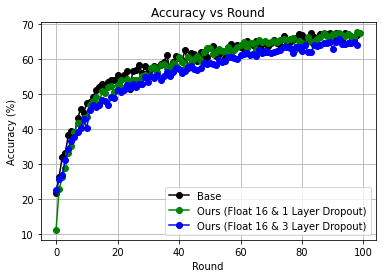
\includegraphics[width=\linewidth, height=0.7\linewidth]{img/Acc_Cifar10.png}
    \caption{Accuracy of our method compared with base FedAvg on Cifar10. The plot shows that our validation accuracy is very similar to the base case even when we remove a significant amount of parameters with dropout and quantization.}
    \label{fig:fed_cifar}
  \end{minipage}\hfill % This filler will push the next minipage to the right, creating space between them
  \begin{minipage}{.45\textwidth}
    \centering
    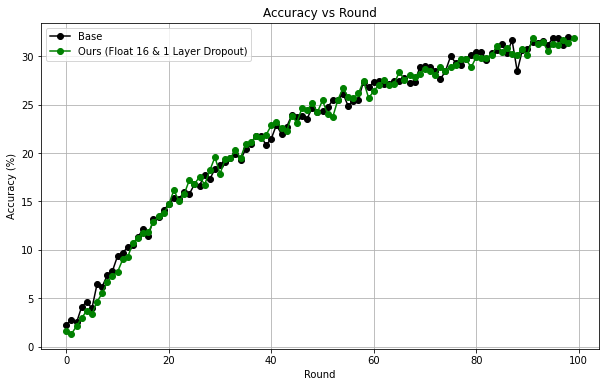
\includegraphics[width=\linewidth, height=0.7\linewidth]{img/Acc_Cifar100.png}
    \caption{Accuracy of our method compared with base FedAvg on Cifar100. The plot shows that our validation accuracy is better than the base case.}
    \label{fig:cifar100}
  \end{minipage}
\end{figure*}

\textbf{Model: }We use a CNN model consisting of one $(3 \times 3)$ convolution layer, followed by a one max-pool and several fully connected layers. We use softmax as an activation in the final layer. For Cifar data sets we use an input size of $(32 \times 32 \times 3)$. This model has a total of 923k trainable parameters. We use validation accuracy as evaluation method. We use TensorFlow for implementation of the models.

\textbf{Hyper-parameters: } We have used Adam optimizer with sparse categorical cross-entropy as loss function. We use the known baseline settings of FedAvg without any changes. Our FL experiments are performed with 10 clients running simultaneouly using the Flower framework.


\begin{figure*}[ht]
  \centering
  \begin{minipage}{.45\textwidth}
    \centering
    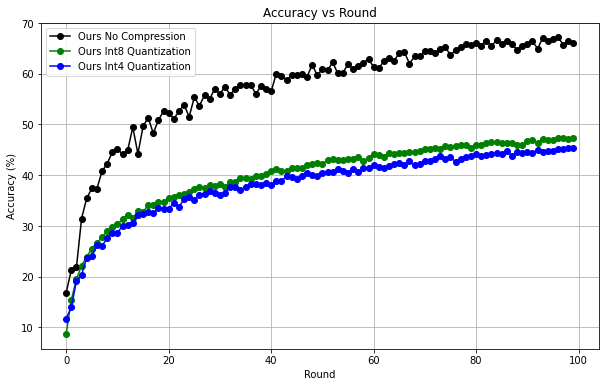
\includegraphics[width=\linewidth, height=0.7\linewidth]{img/Acc_Cifar10_comp.png}
    \caption{Accuracy of our method with different Quantization technique on Cifar10. The plot shows that integer quantization leads to a significant decrease in accuracy.}
    \label{fig:qu_cifar}
  \end{minipage}\hfill % Adding horizontal fill will push the second minipage to the right, creating more space
  \begin{minipage}{.45\textwidth}
    \centering
    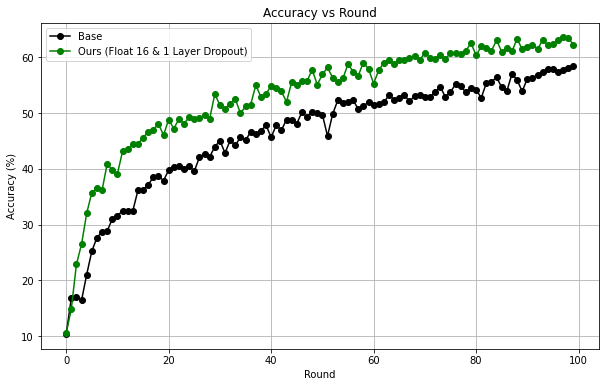
\includegraphics[width=\linewidth, height=0.7\linewidth]{img/Acc_Cifar10_Imb.png}
    \caption{Accuracy of our method compared with base FedAvg on Imbalanced Cifar10. The plot shows that our method provides an advantage over FedAvg in cases of class imbalance while significantly reducing communication needs.}
    \label{fig:imb_cifar}
  \end{minipage}
\end{figure*}


\textbf{Quantization: } Our quantization is inspired by previous work of Jacob et al \cite{jacob2018quantization}. We use 'float16' quantization which is able to achieve 2x compression with minimal accuracy loss. Integer quantization is able to get 4x compression but sufferers from significant loss of precision.

\textbf{ACFed dropout: } For the base case our model does not utilize dropout. We compare this with ACFed dropout applied after one fully connected layer and applied after three fully connected layers. We only experiment applying dropout on fully-connected layers, since CNN layers have very few parameters. ACFed dropout has two more hyper-parameters $\alpha$ and $\beta$. We start with a dropout rate of 0.5, use 0.05 as the value of $\beta$, and 0.1 as the value of $\alpha$. Thus, we increase or decrease the dropout rate by 0.05, unless it's equal to 0.9 or 0.1. We plot the changes in dropout rate throughout the training process in Figure \ref{fig:dropout_training}.

We plot the results of Cifar 10 data set with 'float16' quantization (2x compression) and different levels of dropout in Figure \ref{fig:fed_cifar}. Dropout in one layer, combined with quantization, leads to approximately a 3x reduction in communicated parameter size and three layers of dropout with quantization leads to approximately a 4x reduction in parameter size. The results for Cifar100, presented in Figure \ref{fig:cifar100} show our method achieves similar results across different data sets. 

\textbf{Robustness to class Imbalance: }To test the robustness to imbalanced data we use imbalanced Cifar10 with the number of samples for class 0 and 1 reduced by half. The results of imbalanced cifar10 are plotted in Figure \ref{fig:imb_cifar}. These results show our method provides an advantage over FedAvg in case of imbalanced data set. The dropout rate increases for clients with data from a greater count of majority classes and works as a regularization.

\begin{figure*}[ht]
  \centering
  \begin{minipage}{.45\textwidth}
    \centering
    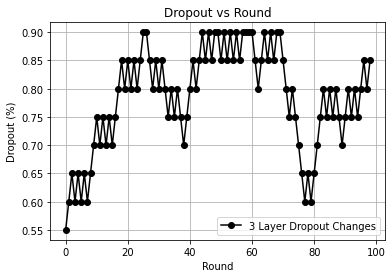
\includegraphics[width=1.1\linewidth, height=.7\linewidth]{img/Drop_Round.png}
    \caption{Change in dropout rate throughout the training process. The average dropout during the training is 0.78.}
    \label{fig:dropout_training}
  \end{minipage}\hfill
  \begin{minipage}{.45\textwidth}
    \centering
    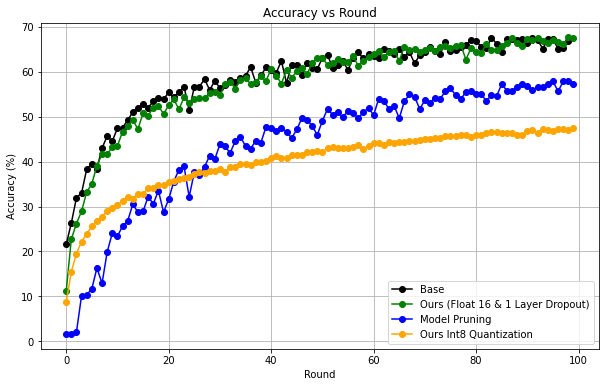
\includegraphics[width=\linewidth, height=0.7\linewidth]{img/comp.png}
    \caption{Comparison of our method with Model Pruning. The plot shows that our emthod achieves better accuracy than Model pruning in case of float 16 compression with dropout.}
    \label{fig:comp_pruning}
  \end{minipage}
\end{figure*}


Model pruning is often used to reduce communication cost in Federated learning \cite{vahidian2021personalized,jiang2022model,zhang2022fedduap}. We compare our method to model pruning as described Jiang et al \cite{jiang2022model} and show the results in Figure \ref{fig:comp_pruning}. Finally, we have a table showing the reduction in communication cost compared to the accuracy of the model in the Table \ref{tab:tab}.

\begin{table}[ht]
\centering
\caption{Comparison of Different Methods for Federated Learning on Cifar10 after 100 round of training. We achieve better accuracy than base model with with adaptive dropout due to better generalization. Combined with float 16 compression we reduce communication cost by 7.2x while having similar accuracy. Integer quantization reduces communication cost significantly but suffers from lower accuracy.}
\label{tab:method_comparison}
\begin{tabular}{|l|c|c|c|}
\hline
\textbf{Dropout Amount} & \textbf{Comm. Cost Reduction} & \textbf{Compression} & \textbf{Accuracy} \\ \hline
Base Model 7.7M params & x & None & 63.87 \% \\ \hline
Adaptive Dropout 1 layer & 3.6x (approx.) & None & 66.03\% \\ \hline
Adaptive Dropout 1 layer & 7.2x (approx.)&Float16 & 65.61\% \\ \hline
Adaptive Dropout 3 layers & 9x (approx.) & Float16 & 60.54\%\\\hline
Model Pruning & 4x (approx.) & None & 55.69\%  \\ \hline
Adaptive Dropout 1 layer & 14.4x (approx.) & Int8 & 47.17\% \\ \hline
\end{tabular}
\label{tab:tab}
\end{table}


\textbf{Limitations}
Our study assumes all clients involved in the FL network are capable of meeting the computational requirements necessary for efficient algorithm performance. This assumption might not accurately reflect the varied capabilities of devices in practical, real-world applications and could skew the model's performance metrics. To counteract the risk of over-fitting, we employed multiple datasets, namely datasets Cifar10 and Cifar100. Utilizing multiple datasets assists the verification that our model's efficacy is generalizable and not over-fitted to specific data characteristics. Using quantization leads to some loss of precision and that might introduce domain adaptation problem in some use cases. 

\section{Conclusion}

Federated learning is dependent on client device performance and communication bandwidth. Both of these can vary a lot based on different demographic groups and thereby exclude people from training models. Research on dropout and quantization methods can address this problem and improve the application of FL. Our work can lead to massive reduction in communication overheads while still being robust to class imbalance issue. To address these issues more, in future we plan to work on client sampling and investigate the use of heterogeneous models in FL.

\bibliographystyle{splncs04}
\bibliography{main}
\end{document}